\documentclass[11pt]{amsart}
\usepackage[centering,margin=2.5cm,a4paper]{geometry}
\usepackage{amssymb}
\usepackage{tikz}
\usepackage{enumerate}
\usepackage{color}
\usepackage{soul}
\theoremstyle{plain}
\newtheorem{theorem}{Theorem}[section]
\newtheorem{lemma}[theorem]{Lemma}
\newtheorem{corollary}[theorem]{Corollary}
\newtheorem{proposition}[theorem]{Proposition}
\newtheorem{fact}[theorem]{Fact}
\newtheorem{observation}[theorem]{Observation}
\newtheorem{claim}[theorem]{Claim}
\theoremstyle{definition}
\newtheorem{definition}[theorem]{Definition}
\newtheorem{example}[theorem]{Example}
\newtheorem{conjecture}[theorem]{Conjecture}
\newtheorem{open}[theorem]{Open Problem}
\newtheorem{problem}[theorem]{Problem}
\newtheorem{question}[theorem]{Question}
\theoremstyle{remark}
\newtheorem{remark}[theorem]{Remark}
\newtheorem{note}[theorem]{Note}
\newtheorem{notation}[theorem]{Notation}
\newtheorem{case}{Case}
\newtheorem{subcase}{Case}[case]

\title[Codimension two and three Kneser Transversals]{Codimension two and three Kneser Transversals}
\thanks{Supported by the ECOS-Nord project M13M01, by CONACyT project 166306, by CONACyT grant 277462 and by PAPIIT-UNAM project IN112614}
\author[\tiny J.~Chappelon]{J.~Chappelon}
\address{Institut Montpelli\'{e}rain Alexander Grothendieck, Universit\'{e} de Montpellier, Case Courrier 051, Place Eug\`{e}ne Bataillon, 34095 Montpellier Cedex 05, France}
\email[Corresponding author]{jonathan.chappelon@umontpellier.fr}
\author[L.~Mart\'{i}nez-Sandoval]{L.~Mart\'{i}nez-Sandoval}
\address{Instituto de Matem\'{a}ticas, Universidad Nacional Aut\'{o}noma de M\'{e}xico, Ciudad Universitaria, M\'{e}xico D.F., 04510, Mexico}
\email{leomtz@im.unam.mx}
\author[L.~Montejano]{L.~Montejano}
\address{Instituto de Matem\'{a}ticas, Universidad Nacional Aut\'{o}noma de M\'{e}xico, Ciudad Universitaria, M\'{e}xico D.F., 04510, Mexico}
\email{luis@math.unam.mx}
\author[L.P.~Montejano]{L.P.~Montejano}
\address{Institut Montpelli\'{e}rain Alexander Grothendieck, Universit\'{e} de Montpellier, Case Courrier 051, Place Eug\`{e}ne Bataillon, 34095 Montpellier Cedex 05, France}
\email{lpmontejano@gmail.com}
\author[J.L.~Ram\'{i}rez Alfons\'{i}n]{J.L.~Ram\'{i}rez Alfons\'{i}n}
\address{Institut Montpelli\'{e}rain Alexander Grothendieck, Universit\'{e} de Montpellier, Case Courrier 051, Place Eug\`{e}ne Bataillon, 34095 Montpellier Cedex 05, France}
\email{jorge.ramirez-alfonsin@umontpellier.fr}
\subjclass[2010]{52A35, 52C40, 52B55, 68-04}
\keywords{transversals, oriented matroids, cyclic polytope}
\date{January 4, 2016}
\begin{document}
\begin{abstract}
Let $k,d,\lambda\geqslant1$ be integers with $d\geqslant\lambda $. In \cite{ABMR}, the following function was introduced:
\par\smallskip
$m(k,d,\lambda)\overset{\mathrm{def}}{=}$ the maximum positive integer $n$ such that every set of $n$ points (not necessarily in general position) in $\mathbb{R}^{d}$ has the property that the convex hulls of all $k$-sets have a common transversal $(d-\lambda)$-plane.
\smallskip\par
This is a continuation of the  recent work \cite{CMMMR} in which it is  introduced and studied  a natural discrete version of $m$ by considering the existence of \emph{complete Kneser transversals} (i.e., $(d-\lambda)$-transversals $L$ to the convex hulls of all $k$-sets and $L$ containing $(d-\lambda)+1$ points of the given set of points).
\smallskip

In this paper, we introduce and study the notions of {\em stability} and {\em unstability}. We give results when $\lambda =2,3$, among other results, we present a classification of (complete) Kneser transversals. These results lead us to new upper and lower bounds for $m$. Finally, by using oriented matroid machinery, we present computational results concerning (complete) Kneser transversal in some special cases. 
\end{abstract}
\maketitle
\section{Introduction}
Let $k,d,\lambda {\geqslant} 1$ be integers with $d, k {\geqslant} \lambda $. Let $m(k,d,\lambda )$ be the maximum positive integer $n$ such that every set of $n$ points (not necessarily in general position) in $\mathbb{R}^{d}$ has the property that the convex hulls of all $k$-sets have a transversal $(d-\lambda )$-plane.
\smallskip

This function was introduced in \cite{ABMR} where it was proved that

\begin{equation}\label{ineq1}
 d-\lambda +k+\left\lceil \frac{k}{\lambda }\right\rceil -1 {\leqslant} m(k,d,\lambda )< d+2(k-\lambda)+1.
\end{equation}
 
The proof of the lower bound follows the same spirit of Dolnikov \cite{D} and uses Schubert calculus in the cohomology ring of Grassmannian manifolds. The value of $m(k,d,\lambda )$ is strongly connected with  the Rado's central Theorem \cite{Rado}.  Indeed, let $n,d,\lambda {\geqslant} 1$ be integers with $d  {\geqslant} \lambda $ and let

\smallskip
\noindent {\bf $\tau(n,d,\lambda )$}$\overset{\mathrm{def}}{=}$ the maximum positive integer $\tau$ such that for any collection $X$ of $n$ points in $\mathbb{R}^{d}$, there is a  $(d-\lambda )$-plane $L_X$ such that any closed half-space $H$ through $L_X$ contains at least $\tau$ points.
\smallskip

We thus have have that $n-\tau(n,d,\lambda)+1$ is equal to the minimum positive integer $k$ such that for any collection $X$ of $n$ points in $\mathbb{R}^{d}$  there is a common transversal $(d-\lambda )$-plane to the convex hulls of all $k$-sets, which is essentially $m(k,d,\lambda)$. Therefore, any improvement to the  lower or upper bounds for $m(d,\lambda, k)$ will give important insight on the above interesting problem.
\medskip

The case when $\lambda=1$ is of particular interest. In \cite{ABMR} it was proved that  $m(k,d,1)=d+2k-2$ and showed that this equality is equivalent to the fact that the chromatic number of the {\em Kneser} graph $KG(n,k)$ is $n-2k+2$, the well-known Kneser's conjecture originally proved by Lov\'asz \cite{L}.  
\medskip

One of the purpose of this paper is to improve upper and lower bounds for $m(k,d,\lambda)$ when $\lambda=2,3$.
\smallskip

From the inequalities in \eqref{ineq1} it can be deduced that

\begin{equation}\label{eq2}
m(k,d,\lambda ) = d-\lambda +k+\left\lceil \frac{k}{\lambda }\right\rceil -1 \text{ for } \lambda=1, k-\lambda{\leqslant} 1 \text{ and } k{\leqslant} 3.
\end{equation}

Furthermore, the equality also holds for $d=\lambda$ \cite[Theorem 6]{ABMR}. In this paper, we shall focus our attention to the case when $d >\lambda {\geqslant} 2$  and  $k-\lambda{\geqslant} 2$.  
\medskip

In \cite{CMMMR} was introduced and studied a natural discrete version of the function $m(k,d,\lambda)$. Let $k,d,\lambda {\geqslant} 1$ be integers with $d{\geqslant} \lambda $ and let $X\subset{\mathbb{R}}^{d}$ be a finite set. A $(d-\lambda)$-plane transversal $L$ to the convex hull of all $k$-sets of $X$ is called \emph{Kneser transversal} . If in addition $L$ contains $(d-\lambda)+1$ points of $X$, then $L$ is a called \emph{complete Kneser} transversal. 
\medskip

It turns out that the existence of a Kneser transversal is not an invariant of the order type. For example, for $d=2$ and $X$ the vertex set of a regular hexagon then the center is a $0$-plane transversal to the convex hull of the $4$-sets. But, by a suitable (slighly) perturbation of these $6$ points we lose this property. The situation is different for complete Kneser transversals. Indeed, it seems that the existence of a complete Kneser $(d-\lambda)$-transversal to the convex hull of the $k$-sets is an invariant of the order type. This naturally lead us to consider the notions of {\em stability} and {\em unstability}. A Kneser transversal is said to be {\em stable} (resp. {\em unstable}) if the given set of points can be slightly perturbed such that the new configuration of points admits (if there is any) only complete Kneser transversals (resp. the new configuration of points do not admit a Kneser transversal). 
\medskip

In the next section, we present an unstability result when $\lambda =2,3$ (Theorem~\ref{stability}). The proof of the latter uses a classification result of Kneser transversal in codimensions 2 and 3  (Theorem~\ref{th:kt}). 
\medskip

In Section~\ref{sec:bound}, we give an upper bound (Theorem~\ref{th:bound}) when $\lambda=2,3$, $(k-\lambda){\geqslant} 2$ and $d{\geqslant} 2(\lambda-1)$. Also, by using results due to Bukh, Matousek and Nivasch \cite{BMN}, we obtain a lower bounds for $m(k,d,2)$ (Equation~\eqref{eq3}).
\medskip

Finally, in Section~\ref{computer}, we present some computational results concerning  the existence of (complete) Kneser transversal lines to the convex hull of the $4$-sets for configurations of $7$ points in $\mathbb{R}^{3}$. This is done by using oriented matroid machinery.

\section{Stability}

Our main result in this section is the following

\begin{theorem}\label{stability}
Let $\epsilon >0$ and let $X=\{x_1,\dots ,x_n\}$ be a finite collection of points in ${\mathbb{R}}^{d}$. Suppose $n=d + 2(k-\lambda)$, $k-\lambda {\geqslant} 2$ and $\lambda=2,3$. Then, there exists $X^\prime=\{x^\prime_1,\dots ,x^\prime_n\}$, a collection of points in ${\mathbb{R}}^{d}$  in general position such that $\mid x_i - x^\prime _i \mid < \epsilon$, for every $i=1,\dots ,n$, and with the property that every transversal $(d-\lambda)$-plane to the convex hull of the $k$-sets of $X^\prime$ is complete (i.e,  it contains  $d-\lambda +1$ points of $X^\prime)$.
\end{theorem}

Before proving Theorem \ref{stability}, we need the following some results.
\medskip

Let $X$ be a collection of points and let $\{L_1, \dots , L_s \}$ be a collection of lines  in $\mathbb{R}^{d}$. We say that $X$ and  $\{L_1, \dots , L_s \}$ are in general position if $\bigcup_{1{\leqslant} i{\leqslant} s}\{a_i, b_i\} \cup X$ is a collection of points in general position, whenever $\{a_i, b_i\} \subset L_i$, for every ${1{\leqslant} i{\leqslant} s}$.

\begin{lemma}\label{lem1}
Let $X$ be a collection of $d-2(\lambda-1)$ points and let $\{L_1, \dots , L_\lambda \}$ be a collection of $\lambda{\geqslant} 1$ lines in general position in $\mathbb{R}^{d}$ with $d{\geqslant} 2(\lambda-1)$.  Then, there is a unique $(d-\lambda)$-plane through $X$ transversal to $\{L_1, \dots , L_\lambda \}$.
\end{lemma}

\begin{proof}
We use induction on $\lambda$. The statement is clearly true for $\lambda=1$. Let us suppose that the result holds for $\lambda-1$ and we prove it for $\lambda$. Consider $H$ the hyperplane generated by $X$ and $\{L_2, \dots , L_\lambda \}$. Then $\lambda_1\cap H$ consist of exactly one point $\{x\}$. Apply now the theorem for the collection of points $X\cup\{x\}$ and the collection of lines $\{L_2, \dots , L_\lambda \}$ in the affine $(d-1)$-space $H$. 
\end{proof}

The following technical lemma will be crucial for the codimension three case in our stability result.

\begin{lemma}\label{lem2}
Let $X \subset \mathbb{R}^{3}-\{0\}$  be a finite set of points and let $\Omega$ be a collection of triples of $X$ satisfying : 
\begin{enumerate}[i)]
\item
for every triple $\{x,y,z \} \in \Omega$ the triangle with vertices $\{x,y,z \}$ contains the origin in its interior, 
\item
the intersection of any two triples of $\Omega$ contains at most one point.
\end{enumerate}
Moreover, suppose that for every $x \not= y \in X$ there is $T \in \Omega$ such that  $\{x,y \} \subset T$.  Then, $X$ is contained in a 2-plane.
\end{lemma}

\begin{proof}
Let $\{a,b,c\} \in \Omega$ and let $H$ be the 2-plane through the origin containing $\{a,b,c\}$. Let $G\subset X$ be the points of $X$ lying on one side of $H$ and $G^\prime$ the points of $X$ on the other side of $H$. By hypothesis, there is a bijection $f:G \to G^\prime $ such that for every point of $x\in G$ there is a point $f(x) \in G^\prime$ with $\{a,x,f(x)\}\in \Omega$. Let $n=\mid G\mid =\mid G^\prime\mid$. Furthermore, for every $\{x,y \}\subset G$ there is $\psi(x,y)\in G^\prime$ such that $\{x,y,\psi(x,y) \}\in \Omega$. For every pair  $\{x,y \}$ of $G$ consider the two edges $(x,\psi(x,y) )$ and $(y,\psi(x,y))$. Since the intersection of any two triples of $\Omega$ contains at most one point we have that if  $\{x^\prime,y^\prime \}\notin \{x,y \}$, then the four edges  $$(x,\psi(x,y) ), (y,\psi(x,y)), (x^\prime,\psi(x^\prime,y^\prime) ), (y^\prime,\psi(x^\prime,y^\prime))$$ are different.  Similarly, for every $\{x,y \}\subset G^\prime$ there is $\psi(x,y)\in G$ such that $\{x,y,\psi(x,y) \}\in \Omega$. If we consider two different pairs of $G^\prime$,   $\{x^\prime,y^\prime \}\notin \{x,y \}$, then the four edges  $$(x,\psi(x,y) ), (y,\psi(x,y)), (x^\prime,\psi(x^\prime,y^\prime) ), (y^\prime,\psi(x^\prime,y^\prime))$$ are different. Furthermore, if $\{x^\prime,y^\prime \}$ is a pair of $G^\prime$ and $\{x,y \}$ is a pair of $G$, then the four edges  $$(x,\psi(x,y) ), (y,\psi(x,y)), (x^\prime,\psi(x^\prime,y^\prime) ), (y^\prime,\psi(x^\prime,y^\prime))$$ are different. This implies that we have at least  4 ${ n \choose 2 }$ edges between $G$ and $G^\prime$ which is impossible if $n >2$.  Furthermore, it is straightforward to show that $n \not= 1,2$.  Hence $X\subset H$. 
\end{proof}

The following result classify Kneser transversals for codimensions 2 and 3.

\begin{theorem}\label{th:kt}
Let $X=\{x_1, x_2, \dots x_n\}$  be a collections of $n=d+2(k-\lambda)$ points in general position in $\mathbb{R}^{d}$. Suppose that $L$ is a $(d-\lambda)$-plane transversal to the convex hulls of all $k$-sets of $X$ with $\lambda=2, 3$ and $k{\geqslant} \lambda +2$ and $d{\geqslant} 2(\lambda-1)$.  Then, either 
\begin{enumerate}[1)]
\item
$L$ is a complete Kneser transversal (i.e., it contains $d-\lambda+1$ points of $X$) or  
\item
$\mid L\cap X \mid= d-2(\lambda-1)$ and the other $2(k-1)$ points of $X$ are matched in $k-1$ pairs in such a way that $L$ intersects the corresponding closed segments determined by them.
\end{enumerate}
\end{theorem}

\begin{proof}
{\em Case 1)}  $\lambda=2$. Since $X$ is in general position, there is a point $x\in X$ which is not in $L$.  Let $H$ be the hyperplane generated by $L$ and $x$. By general position there are at most $d$ points in $H$. Since $L$ is a  transversal to the convex hulls of all $k$-sets of $X$, then at each side of $H$ there are at most $k-2$ points. The fact that $X$ has $d+2(k-2)$ points implies that $H$ has exactly $d$ points of $X$ and there are exactly $k-2$ points at each side of $H$.  Note now that $L$ is a hyperplane of $H$. If in one of the halfspaces of $H$ determined by $L$ there are two points of $X$, then these two points together with the $k-2$ points outside $H$, but in the same side, give rise to a $k$-set whose convex hull does not intersect $L$. This implies that either $L$ is a complete Kneser transversal or that  there are precisely $d-2$ points of $X$ in $L$. Furthermore,  there is  $y\in X\cap H-L$ such that the closed segment determined $x$ and $y$ intersect $L$.  By repeating the same argument with the other $2(k-2)$ points of $X$ outside $H$, we obtain the desired conclusion.
\medskip

{\em Case 2)} $\lambda=3$.  We start by proving that $\mid X\cap L\mid \not= d-3$. We do so by contradiction, let us assume that $X\cap L=\{a_1,\dots ,a_{d-3}\}$ has exactly $d-3$ points. Let $\Omega$ be the collection of triples $\{x,y,z \}$ of $X-L$ such that the interior of the triangle with vertices  $\{x,y,z \}$ intersects the $(d-3)$-plane $L$ in exactly one point.  Note that  the intersection of any two triples of $\Omega$ contains at most one point, otherwise if $\{x,y,z_1 \}$ and $\{x,y,z_2 \}$ belong to $\Omega$, then $$\{a_1,\dots ,a_{d-3}, x,y,z_1,z_2\}$$ are $d+1$ points of $X$ contained in a plane of dimension $d-1$, contradicting the fact that $F \subset \mathbb{R}^{d}$ lies in general position.
\medskip

{\em Subcase a)} $L$ does not intersect any line generated by points of $X-L$. We shall prove that in this case  given $x \not= y \in X-L$ there is $z\in X-L$ such that the triple $\{x,y,z \}\in\Omega$. Indeed, let $x \not= y \in X-L$.  Then $L, x$ and $y$ generates a hyperplane $H^{d-1}$ of $\mathbb{R}^{d}$.  By general position there are at most $d$ points in $H^{d-1}$. Since $L$ is transversal to the convex hulls of all $k$-sets of $X$, then at each side of $H^{d-1}$ there are at most $k-3$ points. The fact that $X$ has $d+2(k-3)$ points implies that $H^{d-1}$ has exactly $d$ points of $X$ and there are exactly $k-3$ points at each side of $H$. Therefore, there is $z\in (X-L)\cap H^{d-1}$. The triangle with vertices $\{x,y,z \}$ intersects $L$, otherwise the $k-3$ points of $X$ on one side of $H$ plus $x, y$ and $z$ give rise to a $k$-set of $X$ that avoids $L$. Finally The triangle with vertices $\{x,y,z \}$ intersect $L$ because $L$ does not intersect any line generated by points of $X-L$. With this we have proved that given $x \not= y \in X-L$ there is $z\in X-L$ such that the triple $\{x,y,z \}\in\Omega$.
\smallskip

Let $L^\perp$ be the 3-dimensional plane through the origen orthogonal to $L$ and let $\pi:\mathbb{R}^{d}\to L^\perp$ be the orthogonal projection.  Let $X^\prime = \pi (X-L)$ and let $\Omega^\prime$ be the collection of triples of $X\prime$ consisting of sets  $\{\pi(x),\pi(y),\pi(z) \}$ for which  $\{x,y,z\}\in \Omega$. By Lemma \ref{lem2}, $X^\prime$ lies in a two dimensional plane of $L^\perp$ and hence  $X$ lies in a hyperplane of  $\mathbb{R}^{d}$ contradicting  the fact that $X$ is in general position.
\medskip

{\em Subcase b)} Assume there are $a,b \in X-L$ such that $L$ intersect the line through $a$ and $b$. By general position  $L$ does not intersect any line generated by points of $X-(L\cup \{a,b \})$. Following the proof of the first case it is possible to prove that $X-(L\cup\{a,b\})$ lies in a hyperplane of  $\mathbb{R}^{d}$ contradicting  the fact that $X$ is in general position. 
\smallskip

This implies that if $L$ is not a complete  Kneser transversal, then $L$ has at least $d-4$ points of $X$. In this case, since $X$ is in general position, there is a point $x\in X$ which is not in $L$.  Let $H^\prime$ be the $(d-2)$-dimensional plane generated by $L$ and $x$. Again by general position, there is a point  $y\in X$ which is not in $H^\prime$. Let $H$ be the hyperplane generated by $L$ and $x$ and $y$. By our previous arguments, $H$ has exactly $d$ points of $X$ and there are exactly $k-3$ points at each side of $H$.   Note that $L$ is transversal to every triangle of  $X\cap H-L$, otherwise, these three points together with the $k-3$ points outside $H$, but in the same side, give rise to a $k$-set whose convex hull does not intersect $L$. This implies that we have exactly 4 points $T=\{t_1,t_2,t_3,t_4\}$ of $X$ in $H$ which are not in $L$ and also that  the points of $T$ are matched  in two pairs in such a way that $L$ intersects the corresponding closed segments determined by them. By repeating the same argument with the other $2(k-3)$ points of $X$ outside $H$, we obtain the desired conclusion.
\end{proof}

We may now prove Theorem~\ref{stability}.

\begin{proof}[Proof of Theorem~\ref{stability}]
Let  $[n]=\{1, \dots,n\}$  and let $\binom{[n]}{s}$ be the collection of all subsets of $X$ of size $s$. Finally, denote by $\Omega$  the finite set of partitions of $[d + 2(k-\lambda)]$ of the form $[d + 2(k-\lambda)]=B_1\sqcup B_2\sqcup \dots \sqcup B_k$, where $\mid B_1 \mid = d-2(\lambda-1)$ and $\mid B_i \mid = 2$, for every $2{\leqslant} i {\leqslant} k$.
\medskip

Let $\Im_X$ be the collection of $(d-\lambda)$-plane transversal to the convex hulls of all $k$-sets of $X$. Let us first note that $\Im_X$ is finite. For this, let $\phi_X:\Im \to \Omega \cup \binom{[n]}{d-\lambda +1}$ defined as follows:
If $L$ is a complete $(d-\lambda)$-plane transversal to the convex hulls of all $k$-sets of $X$, then $\mid X\cap L\mid = d-\lambda +1$, so $\phi_X(L)\in \binom{[n]}{d-\lambda +1}$ is the corresponding set of indices for $X\cap L$. If $L$ is not a complete Kneser transversal, then by Theorem \ref{th:kt}, $\mid L\cap X \mid= d-2(\lambda-1)$ and the other $2(k-1)$ points of $X$ are matched in $k-1$ pairs in such a way that $L$ intersects the corresponding closed segments determined by them, so $\phi_X(L)\in \Omega$ is the corresponding  element of $\Omega$. Clearly, by Theorem \ref{th:kt}, $\phi_X:\Im \to \Omega \cup \binom{[n]}{d-\lambda +1}$ is well defined. Moreover, by Lemma \ref{lem1}, $\phi_X$ is injective.
\medskip

Note now that is if $\alpha \in (\Omega$  $\cup \binom{[n]}{d-\lambda +1}-$ Image $\phi_X)$, then there is $\epsilon >0$ with the property that if $X^\prime=\{x^\prime_1,\dots ,x^\prime_n\}$, is a collection of points in ${\mathbb{R}}^{d}$  in general position such that $\mid x_i - x^\prime _i \mid < \epsilon$, for every $i=1,\dots ,n$, then $\alpha \in (\Omega \cup \binom{[n]}{d-\lambda +1}-$ Image $\phi_{X^\prime}$. Moreover, by Lemma \ref{lem1}, since $k-\lambda {\geqslant} 2$, given $\epsilon >0$ and  $\alpha \in \Omega$  $ \cap $ Image $\phi_X$, there is $X^\prime=\{x^\prime_1,\dots ,x^\prime_n\}$ in general position, with $\mid x_i - x^\prime _i \mid < \epsilon$ and such that $\alpha \notin$ Image $\phi_{X^\prime}$. To see this, we may assume without loss of generality that
$$
\alpha= \{ 1, \dots ,d-2(\lambda-1)\}, \{d-2\lambda +3, d-2\lambda+4\}, \dots , \{d+2k+2\lambda-1, d+2k-2\lambda\}
$$
and $L$ is a $(d-\lambda)$-plane that contains $\{ x_1, \dots ,x_{d-2(\lambda-1)}\}$ and intersects the $k-1$ closed segments with extreme points
$$
\{x_{d-2\lambda +3}, x_{d-2\lambda+4}\}, \dots ,  \{x_{d+2k+2\lambda-1}, x_{d+2k-2\lambda}\}.
$$
By Lemma~\ref{lem1}, since $k-2{\geqslant} \lambda$, we may chose $x^{\prime}_{d+2k-2\lambda}$ such that $\mid x_{d+2k-2\lambda}-x^{\prime}_{d+2k-2\lambda}\mid<\epsilon $ and in such a way that there is not a $(d-\lambda)$-plane that contains $\{ x_1, \dots ,x_{d-2(\lambda-1)}\}$ and intersects the $k-1$ closed segments with extreme points
$$
\{x_{d-2\lambda +3}, x_{d-2\lambda+4}\}, \dots ,  \{x_{d+2k+2\lambda-1}, x^{\prime}_{d+2k-2\lambda}\}
$$

This implies that we can chose $X^\prime=\{x^\prime_1,\dots ,x^\prime_n\}$, a collection of points in ${\mathbb{R}}^{d}$  in general position sufficiently close to $X$ and with the property that Image $\phi_{X^\prime} \subset \binom{[n]}{d-\lambda +1}$ and hence admits only complete Kneser transversals.
\end{proof}

We believe that Theorem~\ref{stability} is also true for $\lambda{\geqslant} 3$ but the proof needs a more difficult and complicated version of Theorem~\ref{th:kt}.

\section{Bounds for $m(k,d,\lambda)$ when $\lambda=2,3$}\label{sec:bound}

We start by proving the following upper bound

\begin{theorem}\label{th:bound}
Let $\lambda=2,3$, $k-\lambda {\geqslant} 2$ and $d{\geqslant} 2(\lambda-1)$. Then,
$$
m(k,d,\lambda)<d+2(k-\lambda).
$$
\end{theorem}

\begin{proof}
Let $X=\{x_1,\dots ,x_n\}$ be a finite collection of points in ${\mathbb{R}}^{d}$ embedded in the momentum curve. By Theorem 2,  there exist $X^\prime=\{x^\prime_1,\dots ,x^\prime_n\}$, a collection of points in ${\mathbb{R}}^{d}$  in general position with the order type of the cyclic polytope  and with the property that every transversal $(d-\lambda)$-plane to the convex hull of the $k$-sets of $X^\prime$ is complete (i.e,  contains  $d-\lambda +1$ points of $X^\prime)$. By \cite[Theorem 1.2]{CMMMR}, also $X^\prime$ does not admit  a complete transversal. Therefore,  there exist a collection of  $d+2(k-\lambda)$ point in ${\mathbb{R}}^{d}$ without $(d-\lambda)$-plane transversal to the convex hull of the $k$-sets, and hence $m(k,d,\lambda)<d+2(k-\lambda)$.
\end{proof}

In dimension three, when $k{\geqslant} 6$, a better upper bound was proved by Tancer \cite{T}. In fact, it is possible to embed $2k-2$ points in general position in $3$-space on the moment curve in the first two dimensions and a quickly growing function in the third dimension in such a way that there is not  a transversal line to the convex hull of the $k$-sets.
\medskip

For a codimension two lower bound, we need the following result due Bukh, Matousek and Nivash \cite{BMN} that was proved by using equivariant topology.

\begin{quote}
Let $X=\{x_1, x_2, \dots x_n\}$  be a collections of $n$ points in $\mathbb{R}^{d}$.  Then there is a codimension two affine plane $L$ and $2d-1$ hyperplanes passing through $L$ that divide $\mathbb{R}^{d}$ into $4d-2$ parts, each containing at most $\frac{n}{4d-2} + O(n)$ points of $X$.
\end{quote}

This implies that every hyperplane $H$ through $L$ leaves at least $\frac{(2d-2)n}{4d-2}$ points of $X$ at each side of $H$ and thus
$$
\left\lfloor \frac{(2d-2)n}{4d-2}\right\rfloor{\leqslant} \tau(k,d,2).
$$
Furthermore, if $k{\geqslant}  \frac{(4d-2)n}{2d}$,  the codimension two affine plane $L$ intersect the convex hull of every $k$-set of $X$. This implies that

\begin{equation}\label{eq3}
\left\lceil \frac{(4d-2)k}{2d}\right\rceil{\leqslant} m(k,d,2).
\end{equation}

From Equation~\eqref{eq3} and Theorem~\ref{th:bound} we obtain 
$$
2-\frac{1}{d}{\leqslant} \lim_{k\to\infty}\frac{m(k,d,2)}{k} < 2.
$$
Therefore, for $d{\geqslant}3, \lambda=2$ and $k$ large enough the conjectured value \cite[Conjecture 1]{ABMR} 
$$
m(k,d,\lambda )=d-\lambda +k+\left\lceil \frac{k}{\lambda }\right\rceil -1
$$
is false.

\section {Computational results}\label{computer}

A \emph{point configuration} (or affine point configuration) is a finite set of points in Euclidean $d$-space. An \emph{abstract order type} is the relabeling class of an acyclic oriented matroid. The abstract order types of realizable oriented matroids are called {\em order types} and correspond to {\em isomorphism types} of configurations of points.
\medskip

In \cite{ABMR} it is proved that $m(3,2,4)=6$ and also that there is never a transversal line to all tetrahedra formed by any configuration of 8 points in ${\mathbb{R}}^3$, and thus $m(3,2,4)<8$.

\begin{question}
Is there a transversal line to all tetrahedra formed by any configuration of 7 points in ${\mathbb{R}}^3$ ?
\end{question}

We will answer this question by completely classifying Kneser transversals lines for configurations of 7 points in ${\mathbb{R}}^3$. It is known that there are $5083$ abstract order types of rank $r=4$ ($d=3$) of cardinality $n=7$ \cite{F}. Among these $5083$ abstract order types, $246$ of them are in general position (we thus have that in the corresponding oriented matroids any $4$-tuple of elements is a basis and any $5$-tuple of elements is a circuit).

\subsection{Complete Kneser transversal line}

Let $\mathcal{M}=(E,B)$ be a configuration of $7$ points $E:=\{x_1,\ldots,x_7\}$ in general position in ${\mathbb{R}}^3$. The first thing we want to know is whether there exists a complete transversal line to the convex hull of the $4$-subsets of $E$. It is possible to detect when the line joining $x_{i_1}$ and $x_{i_2}$ intersects the interior of the triangle $(x_{i_3},x_{i_4},x_{i_5})$.

\begin{proposition}\label{prop1}
Let $\mathcal{M}=(E,B)$ be a configuration of $7$ points $E:=\{x_1,\ldots,x_7\}$ in general position in ${\mathbb{R}}^3$. The line $(x_{i_1},x_{i_2})$ intersects the interior of the triangle $(x_{i_3},x_{i_4},x_{i_5})$ if and only if $sg(x_{i_3})=sg(x_{i_4})=sg(x_{i_5})$ for the circuit $\{x_{i_1},x_{i_2},x_{i_3},x_{i_4},x_{i_5}\}$ of $\mathcal{M}$.
\end{proposition}

\begin{proof}
Since $\mathcal{M}$ is acyclic, it is not possible that all the elements of the circuit $c:=\{x_{i_1},x_{i_2},x_{i_3},x_{i_4},x_{i_5}\}$ are of the same sign. Moreover, as depicted in Figure~\ref{fig1}, the line $(x_{i_1},x_{i_2})$ intersects the interior of the triangle $(x_{i_3},x_{i_4},x_{i_5})$ if and only if the Radon partition associated to $c$ is one of $\left\{ \left\{ x_{i_1},x_{i_2} \right\} , \left\{ x_{i_3},x_{i_4},x_{i_5} \right\} \right\}$ , $\left\{ \left\{ x_{i_1} \right\} , \left\{ x_{i_2},x_{i_3},x_{i_4},x_{i_5} \right\} \right\}$ or \\
$\left\{ \left\{ x_{i_2} \right\} , \left\{ x_{i_1},x_{i_3},x_{i_4},x_{i_5} \right\} \right\}$.
\end{proof}

\begin{figure}
\begin{center}
\begin{tabular}{cc}
\begin{tikzpicture}
\draw (-0.1,0.1) -- (0.1,-0.1);
\draw (0.1,0.1) -- (-0.1,-0.1);
\draw (-0.1,2.6) -- (0.1,2.4);
\draw (0.1,2.6) -- (-0.1,2.4);
\draw (-0.1,-2.4) -- (0.1,-2.6);
\draw (0.1,-2.4) -- (-0.1,-2.6);
\draw (0,0) -- (0,3);
\draw[dotted] (0,0) -- (0,-5/3);
\draw (0,-5/3) -- (0,-3);
\draw (-3,0) -- (2,1) -- (-1,-3) -- (-3,0);
\node[right] (1) at (0,2.5) {$x_{i_1}$};
\node[right] (2) at (0,-2.5) {$x_{i_2}$};
\node[left] (3) at (-3,0) {$x_{i_3}$};
\node[right] (4) at (2,1) {$x_{i_4}$};
\node[below] (5) at (-1,-3) {$x_{i_5}$};
\end{tikzpicture}
&
\begin{tikzpicture}
\draw (-0.1,0.1) -- (0.1,-0.1);
\draw (0.1,0.1) -- (-0.1,-0.1);
\draw (-0.1,2.6) -- (0.1,2.4);
\draw (0.1,2.6) -- (-0.1,2.4);
\draw (-0.1,1.35) -- (0.1,1.15);
\draw (0.1,1.35) -- (-0.1,1.15);
\draw (0,0) -- (0,3);
\draw[dotted] (0,0) -- (0,-5/3);
\draw (0,-5/3) -- (0,-3);
\draw (-3,0) -- (2,1) -- (-1,-3) -- (-3,0);
\node[right] (1) at (0,2.5) {$x_{i_1}$};
\node[right] (2) at (0,1.25) {$x_{i_2}$};
\node[left] (3) at (-3,0) {$x_{i_3}$};
\node[right] (4) at (2,1) {$x_{i_4}$};
\node[below] (5) at (-1,-3) {$x_{i_5}$};
\end{tikzpicture} \\
$\left\{ \left\{ x_{i_1},x_{i_2} \right\} , \left\{ x_{i_3},x_{i_4},x_{i_5} \right\} \right\}$ & $\left\{ \left\{ x_{i_2} \right\} , \left\{ x_{i_1},x_{i_3},x_{i_4},x_{i_5} \right\} \right\}$
\end{tabular}
\end{center}
\caption{Radon partitions where the line $(x_{i_1},x_{i_2})$ intersects the triangle $(x_{i_3},x_{i_4},x_{i_5})$.}\label{fig1}
\end{figure}

We notice that since the points of $E$ are in general position, then the line $(x_{i_1},x_{i_2})$ cannot intersect the triangle $(x_{i_3},x_{i_4},x_{i_5})$ on a vertex.

For each of the $\binom{7}{2}=21$ couples $(x_{i_1},x_{i_2})$, we determine, by using Proposition~\ref{prop1}, if the line $(x_{i_1},x_{i_2})$ intersects the $\binom{5}{3}=10$ triangles of $E\setminus\{x_{i_1},x_{i_2}\}$. Since the points are in general position, it is easy to see that if $(x_{i_1},x_{i_2})$ intersects a tetrahedron $T$ whose vertices are in $E$, then $(x_{i_1},x_{i_2})$ intersects at least two faces (two triangles) of $T$. Therefore, if $(x_{i_1},x_{i_2})$ intersects the triangle $(x_{i_3},x_{i_4},x_{i_5})$, it intersects the two tetrahedra $(x_{i_3},x_{i_4},x_{i_5},x_{i_6})$ and $(x_{i_3},x_{i_4},x_{i_5},x_{i_7})$, where $\left\{x_{i_1},x_{i_2},x_{i_3},x_{i_4},x_{i_5},x_{i_6},x_{i_7}\right\}=E$. Finally, if the line $(x_{i_1},x_{i_2})$ intersects the $\binom{5}{4}=5$ tetrahedra generated from $E\setminus\{x_{i_1},x_{i_2}\}$, it immediately follows that $(x_{i_1},x_{i_2})$ is transversal to all the tetrahedra of $E$.

For instance, for $\mathcal{M}=OT(7,4,2)$ in the classification given in \cite{F}, that is the abstract order type representing a point configuration having the chirotope $\chi_{\mathcal{M}} : B \rightarrow \{0,-,+\}$ given by
$$
\scriptsize
\begin{array}{ccccccccccccccccccc}
 & 1 & 1 & 1 & 1 & 2 & 1 & 1 & 1 & 2 & 1 & 1 & 2 & 1 & 2 & 3 & 1 & 1 & 1  \\
 & 2 & 2 & 2 & 3 & 3 & 2 & 2 & 3 & 3 & 2 & 3 & 3 & 4 & 4 & 4 & 2 & 2 & 3  \\
 & 3 & 3 & 4 & 4 & 4 & 3 & 4 & 4 & 4 & 5 & 5 & 5 & 5 & 5 & 5 & 3 & 4 & 4  \\
 & 4 & 5 & 5 & 5 & 5 & 6 & 6 & 6 & 6 & 6 & 6 & 6 & 6 & 6 & 6 & 7 & 7 & 7  \\
 \chi_{\mathcal{M}} = & + & - & + & - & - & - & + & - & - & - & + & + & - & - & + & + & - & +  \\
 \\
  & 2 & 1 & 1 & 2 & 1 & 2 & 3 & 1 & 1 & 2 & 1 & 2 & 3 & 1 & 2 & 3 & 4 & \\
 & 3 & 2 & 3 & 3 & 4 & 4 & 4 & 2 & 3 & 3 & 4 & 4 & 4 & 5 & 5 & 5 & 5 & \\
 & 4 & 5 & 5 & 5 & 5 & 5 & 5 & 6 & 6 & 6 & 6 & 6 & 6 & 6 & 6 & 6 & 6 & \\
 & 7 & 7 & 7 & 7 & 7 & 7 & 7 & 7 & 7 & 7 & 7 & 7 & 7 & 7 & 7 & 7 & 7 & \\
 \chi_{\mathcal{M}} = & + & + & - & - & + & + & + & + & - & - & + & - & + & + & + & - & +& \\
\end{array}
$$

the line $L$ going through $1$ and $5$ is complete Kneser transversal line. Indeed, by Proposition~\ref{prop1}, we know that $L$ intersects the triangles $(2,3,4)$, $(2,3,6)$, $(2,6,7)$ and $(3,4,7)$ since the corresponding circuits are
$$
\begin{array}{cccc}
\{\bar{1}2345\}, & \{1\bar{2}\bar{3}5\bar{6}\}, & \{1\bar{2}5\bar{6}\bar{7}\}, & \{1\bar{3}\bar{4}\bar{5}\bar{7}\},\\
\end{array}
$$
implying  that $L$ intersects the $5$ tetrahedra $(2,3,4,6)$, $(2,3,4,7)$, $(2,3,6,7)$, $(2,4,6,7)$ and $(3,4,6,7)$.
\medskip

By applying the above approach, we obtain the following

\begin{theorem}\label{th:comp1}  
Among the $246$ configurations of $7$ points in general position in ${\mathbb{R}}^3$ there are 124 admiting a complete Kneser transversal. These configurations correspond to the 124 realizable rank 4 oriented matroids on 7 elements given in by the following set according to the classification in \cite{F}
{\scriptsize $$
A:=
\begin{array}[t]{l}
\left\{2,3,5,6,8,9,10,15,16,18,20,21,25,27,28,29,33,34,35,38,40,41,43,44,45,46,\right.\\
47,48,50,51,52,55,56,60,62,63,64,67,68,69,70,71,72,74,76,79,85,88,92,93,\\
94,95,96,97,98,99,100,101,102,106,107,109,110,111,112,113,118,120,123,124,\\
125,127,132,134,135,136,140,141,142,144,145,150,151,154,155,156,157,159,\\
160,166,167,171,172,177,178,182,183,184,185,186,187,189,191,192,195,199,\\
\left. 200,201,206,207,208,211,212,219,220,221,224,225,228,229,234,237,243,244\right\}.
\end{array}
$$}
\end{theorem}

\subsection{Kneser Transversal line}

Let $\mathcal{M}=(E,B)$ be a point configuration of $7$ points $E:=\{x_1,\ldots,x_7\}$ in general position in ${\mathbb{R}}^3$. From  Classification Theorem \ref{th:kt}, if there exists a non-complete Kneser transversal line to the convex hull of its $4$-subsets, then the $7$ points of $\mathcal{M}$ must look as illustrated in Figure~\ref{fig2}. This implies that $\mathcal{M}$ admits the following circuits

\begin{eqnarray}\label{eqa}
\{\overline{x_1}\, \overline{x_2}\, x_3\, x_4\, x_7\},
&
\{\overline{x_1}\, \overline{x_2}\, x_5\, x_6\, x_7\},
&
\{\overline{x_3}\, \overline{x_4}\, x_5\, x_6\, x_7\},
\end{eqnarray}

and cocircuits
\begin{eqnarray}\label{eqb}
\{\overline{x_3}\, x_4\, \overline{x_5}\, x_6\},
&
\{\overline{x_1}\, x_2\, x_5\, \overline{x_6}\},
&
\{\overline{x_1}\, x_2\, \overline{x_3}\, x_4\}.
\end{eqnarray}

\begin{figure}
\begin{center}
\begin{tabular}{ccc}
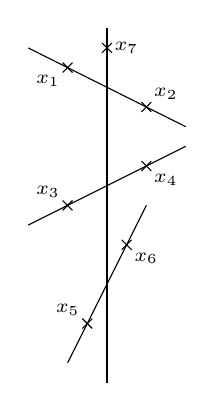
\begin{tikzpicture}[scale=0.25]
\scriptsize
\draw (0,0) -- (0,18);
\draw (-2,1) -- (2,9);
\draw (-4,8) -- (4,12);
\draw (-4,17) -- (4,13);

\draw (-2.25,16.25) -- (-1.75,15.75);
\draw (-1.75,16.25) -- (-2.25,15.75);
\node[below left] (1) at (-2,16) {$x_1$};

\draw (1.75,14.25) -- (2.25,13.75);
\draw (2.25,14.25) -- (1.75,13.75);
\node[above right] (2) at (2,14) {$x_2$};

\draw (-2.25,9.25) -- (-1.75,8.75);
\draw (-1.75,9.25) -- (-2.25,8.75);
\node[above left] (3) at (-2,9) {$x_3$};

\draw (1.75,11.25) -- (2.25,10.75);
\draw (2.25,11.25) -- (1.75,10.75);
\node[below right] (4) at (2,11) {$x_4$};

\draw (-1.25,3.25) -- (-0.75,2.75);
\draw (-0.75,3.25) -- (-1.25,2.75);
\node[above left] (5) at (-1,3) {$x_5$};

\draw (0.75,7.25) -- (1.25,6.75);
\draw (1.25,7.25) -- (0.75,6.75);
\node[below right] (6) at (1,7) {$x_6$};

\draw (-0.25,17.25) -- (0.25,16.75);
\draw (0.25,17.25) -- (-0.25,16.75);
\node[right] (7) at (0,17) {$x_7$};
\end{tikzpicture}
& \quad\quad\quad &
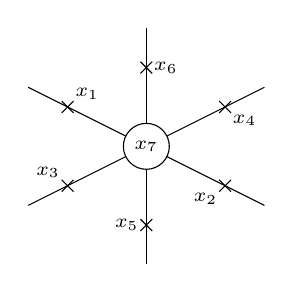
\begin{tikzpicture}[scale=0.5]
\scriptsize
\draw (0,0) -- (0,6);
\draw (-3,1.5) -- (3,4.5);
\draw (3,1.5) -- (-3,4.5);

\draw (-2.15,4.15) -- (-1.85,3.85);
\draw (-1.85,4.15) -- (-2.15,3.85);
\node[above right] (1) at (-2,4) {$x_1$};

\draw (1.85,2.15) -- (2.15,1.85);
\draw (2.15,2.15) -- (1.85,1.85);
\node[below left] (2) at (2,2) {$x_2$};

\draw (-2.15,2.15) -- (-1.85,1.85);
\draw (-1.85,2.15) -- (-2.15,1.85);
\node[above left] (3) at (-2,2) {$x_3$};

\draw (1.85,4.15) -- (2.15,3.85);
\draw (2.15,4.15) -- (1.85,3.85);
\node[below right] (4) at (2,4) {$x_4$};

\draw (-0.15,1.15) -- (0.15,0.85);
\draw (0.15,1.15) -- (-0.15,0.85);
\node[left] (5) at (0,1) {$x_5$};

\draw (-0.15,5.15) -- (0.15,4.85);
\draw (0.15,5.15) -- (-0.15,4.85);
\node[right] (6) at (0,5) {$x_6$};

\node[draw,circle,fill=white] (7) at (0,3) {$x_7$};
\end{tikzpicture} \\
Representation in ${\mathbb{R}}^3$ & & Projection in ${\mathbb{R}}^2$
\end{tabular}
\end{center}
\caption{$7$ points in ${\mathbb{R}}^3$ with circuits and cocircuits satisfying \eqref{eqa} and \eqref{eqb} with a Kneser transversal line to all $4$-sets}\label{fig2}
\end{figure}

However it is possible that certain configurations of $7$ points $\mathcal{M}$ having circuits \eqref{eqa} and cocircuits \eqref{eqa} do not admit a transversal line to the convex hull of its $4$-subsets. For example, if we consider the point configuration represented in Figure~\ref{fig3}.

\begin{figure}
\begin{center}
\begin{tabular}{ccc}
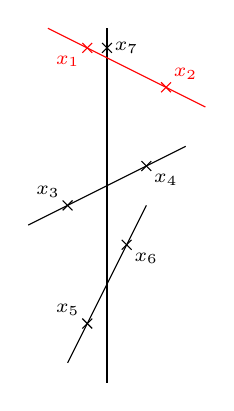
\begin{tikzpicture}[scale=0.25]
\scriptsize
\draw (0,0) -- (0,18);
\draw (-2,1) -- (2,9);
\draw (-4,8) -- (4,12);
\draw[color=red] (-3,18) -- (5,14);

\draw[color=red] (-1.25,17.25) -- (-0.75,16.75);
\draw[color=red] (-0.75,17.25) -- (-1.25,16.75);
\node[color=red,below left] (1) at (-1,17) {$x_1$};

\draw[color=red] (2.75,15.25) -- (3.25,14.75);
\draw[color=red] (3.25,15.25) -- (2.75,14.75);
\node[color=red,above right] (2) at (3,15) {$x_2$};

\draw (-2.25,9.25) -- (-1.75,8.75);
\draw (-1.75,9.25) -- (-2.25,8.75);
\node[above left] (3) at (-2,9) {$x_3$};

\draw (1.75,11.25) -- (2.25,10.75);
\draw (2.25,11.25) -- (1.75,10.75);
\node[below right] (4) at (2,11) {$x_4$};

\draw (-1.25,3.25) -- (-0.75,2.75);
\draw (-0.75,3.25) -- (-1.25,2.75);
\node[above left] (5) at (-1,3) {$x_5$};

\draw (0.75,7.25) -- (1.25,6.75);
\draw (1.25,7.25) -- (0.75,6.75);
\node[below right] (6) at (1,7) {$x_6$};

\draw (-0.25,17.25) -- (0.25,16.75);
\draw (0.25,17.25) -- (-0.25,16.75);
\node[right] (7) at (0,17) {$x_7$};
\end{tikzpicture}
& \quad\quad\quad &
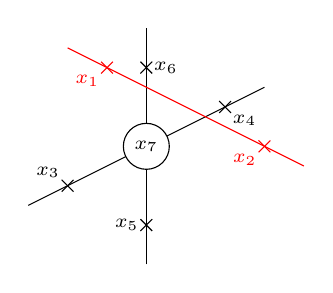
\begin{tikzpicture}[scale=0.5]
\scriptsize
\draw (0,0) -- (0,6);
\draw (-3,1.5) -- (3,4.5);
\draw[color=red] (4,2.5) -- (-2,5.5);

\draw[color=red] (-1.15,5.15) -- (-0.85,4.85);
\draw[color=red] (-0.85,5.15) -- (-1.15,4.85);
\node[color=red,below left] (1) at (-1,5) {$x_1$};

\draw[color=red] (2.85,3.15) -- (3.15,2.85);
\draw[color=red] (3.15,3.15) -- (2.85,2.85);
\node[color=red,below left] (2) at (3,3) {$x_2$};

\draw (-2.15,2.15) -- (-1.85,1.85);
\draw (-1.85,2.15) -- (-2.15,1.85);
\node[above left] (3) at (-2,2) {$x_3$};

\draw (1.85,4.15) -- (2.15,3.85);
\draw (2.15,4.15) -- (1.85,3.85);
\node[below right] (4) at (2,4) {$x_4$};

\draw (-0.15,1.15) -- (0.15,0.85);
\draw (0.15,1.15) -- (-0.15,0.85);
\node[left] (5) at (0,1) {$x_5$};

\draw (-0.15,5.15) -- (0.15,4.85);
\draw (0.15,5.15) -- (-0.15,4.85);
\node[right] (6) at (0,5) {$x_6$};

\node[draw,circle,fill=white] (7) at (0,3) {$x_7$};
\end{tikzpicture}\\
Representation in ${\mathbb{R}}^3$ & & Projection in ${\mathbb{R}}^2$
\end{tabular}
\end{center}
\caption{$7$ points in ${\mathbb{R}}^3$ with circuits and cocircuits satisfying \eqref{eqa} and \eqref{eqb} but without transversal line to all $4$-sets}\label{fig3}
\end{figure}

Nevertheless, we may identify whether a configuration of 7 points admits a Kneser transversal line. For this, let us consider the oriented matroid $\mathcal{M}_8$ associated to the configuration of  $8$ points $E:=\{x_1,\dots,x_8\}$ in ${\mathbb{R}}^3$, not necessarily in general position, given in Figure~\ref{fig4}. The deletion of either point $x_7$ or point $x_8$ from $\mathcal{M}$ yields to a configuration on $7$ points as represented in Figure~\ref{fig2} admiting thus a Kneser transversal line (containing either $x_7$ or $x_8$) to the convex hull of its $4$-subsets. We thus have that the line going through $x_7$ and $x_8$ would be a complete Kneser transversal line of the 8-point configuration. Moreover, any  configuration on $7$ points as represented in Figure~\ref{fig2} arises on this way.

We may thus detect all such configurations $\mathcal{M}_8$. We do this by noticing that an oriented matroid $\mathcal{M}$ is a such configuration if and only if $\mathcal{M}$ admits the following cocircuits

\begin{eqnarray}\label{eqc}
\{\overline{x_3}\, x_4\, \overline{x_5}\, x_6\},
&
\{\overline{x_1}\, x_2\, x_5\, \overline{x_6}\},
&
\{\overline{x_1}\, x_2\, \overline{x_3}\, x_4\}.
\end{eqnarray}

\begin{figure}
\begin{center}
\begin{tabular}{ccc}
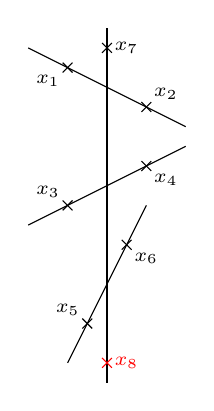
\begin{tikzpicture}[scale=0.25]
\scriptsize
\draw (0,0) -- (0,18);
\draw (-2,1) -- (2,9);
\draw (-4,8) -- (4,12);
\draw (-4,17) -- (4,13);

\draw (-2.25,16.25) -- (-1.75,15.75);
\draw (-1.75,16.25) -- (-2.25,15.75);
\node[below left] (1) at (-2,16) {$x_1$};

\draw (1.75,14.25) -- (2.25,13.75);
\draw (2.25,14.25) -- (1.75,13.75);
\node[above right] (2) at (2,14) {$x_2$};

\draw (-2.25,9.25) -- (-1.75,8.75);
\draw (-1.75,9.25) -- (-2.25,8.75);
\node[above left] (3) at (-2,9) {$x_3$};

\draw (1.75,11.25) -- (2.25,10.75);
\draw (2.25,11.25) -- (1.75,10.75);
\node[below right] (4) at (2,11) {$x_4$};

\draw (-1.25,3.25) -- (-0.75,2.75);
\draw (-0.75,3.25) -- (-1.25,2.75);
\node[above left] (5) at (-1,3) {$x_5$};

\draw (0.75,7.25) -- (1.25,6.75);
\draw (1.25,7.25) -- (0.75,6.75);
\node[below right] (6) at (1,7) {$x_6$};

\draw (-0.25,17.25) -- (0.25,16.75);
\draw (0.25,17.25) -- (-0.25,16.75);
\node[right] (7) at (0,17) {$x_7$};

\draw[color=red] (-0.25,1.25) -- (0.25,0.75);
\draw[color=red] (0.25,1.25) -- (-0.25,0.75);
\node[color=red,right] (8) at (0,1) {$x_8$};
\end{tikzpicture}
& \quad\quad\quad &
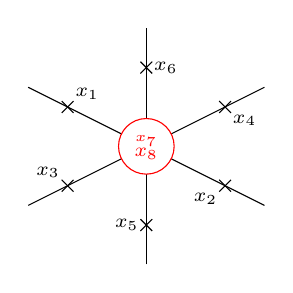
\begin{tikzpicture}[scale=0.5]
\scriptsize
\draw (0,0) -- (0,6);
\draw (-3,1.5) -- (3,4.5);
\draw (3,1.5) -- (-3,4.5);

\draw (-2.15,4.15) -- (-1.85,3.85);
\draw (-1.85,4.15) -- (-2.15,3.85);
\node[above right] (1) at (-2,4) {$x_1$};

\draw (1.85,2.15) -- (2.15,1.85);
\draw (2.15,2.15) -- (1.85,1.85);
\node[below left] (2) at (2,2) {$x_2$};

\draw (-2.15,2.15) -- (-1.85,1.85);
\draw (-1.85,2.15) -- (-2.15,1.85);
\node[above left] (3) at (-2,2) {$x_3$};

\draw (1.85,4.15) -- (2.15,3.85);
\draw (2.15,4.15) -- (1.85,3.85);
\node[below right] (4) at (2,4) {$x_4$};

\draw (-0.15,1.15) -- (0.15,0.85);
\draw (0.15,1.15) -- (-0.15,0.85);
\node[left] (5) at (0,1) {$x_5$};

\draw (-0.15,5.15) -- (0.15,4.85);
\draw (0.15,5.15) -- (-0.15,4.85);
\node[right] (6) at (0,5) {$x_6$};

\node[color=red,draw,circle,fill=white] (7) at (0,3) {$\stackrel{x_7}{x_8}$};
\end{tikzpicture} \\
Representation in ${\mathbb{R}}^3$ & & Projection in ${\mathbb{R}}^2$
\end{tabular}
\end{center}
\caption{$8$ points in ${\mathbb{R}}^3$ with a complete transversal line to all $4$-sets}\label{fig4}
\end{figure}

For each of the $10775236$ order types of $8$ points in ${\mathbb{R}}^3$, we consider a representant $\mathcal{M}$ of this order type. If the configuration $\mathcal{M}$ admits cocircuits of the form \eqref{eqc}, we delete $x_7$ or $x_8$ obtaining configurations of $7$ points in general position as in Figure~\ref{fig2}. We then find an order type for such a configuration of $7$ points admitting a non-complete Kneser transversal line to the convex hull of its $4$-subsets. We obtain the following

\begin{theorem}\label{th:comp2}
Among the $246$ configurations of $7$ points in general position in ${\mathbb{R}}^3$ there are 124  admitting a representation for which there is a non-complete Kneser transversal line to the convex hull of its $4$-subsets. These configurations correspond to the 124 realizable rank 4 oriented matroids on 7 elements given in by the following set according to the classification in \cite{F}
{\scriptsize $$
B :=
\begin{array}[t]{l}
\left\{1,2,4,6,7,10,11,12,13,14,16,19,24,26,29,30,31,32,36,38,39,40,41,42,55,58,\right.\\
59,60,61,62,63,65,70,71,72,74,76,77,78,79,80,81,82,83,85,86,87,88,89,90,\\
91,93,96,97,98,99,101,102,103,104,105,111,114,117,121,122,124,126,128,129,\\
130,138,139,140,145,146,147,148,149,151,152,153,158,165,170,171,172,173,\\
174,175,176,177,180,185,194,196,197,198,199,201,204,206,207,209,211,212,\\
\left. 213,214,215,217,218,219,220,230,235,236,237,238,239,240,241,242,244,246\right\}.
\end{array}
$$}
\end{theorem}

\begin{corollary}
Among the $246$ configurations of $7$ points in general position in ${\mathbb{R}}^3$, $124$ configurations admits a Kneser transversal line to the convex hull of the $4$-subsets 
and $122$ configurations do not admit a Kneser transversal line to the convex hull of their $4$-subsets.
\end{corollary}

\begin{proof} By Theorems \ref{th:comp1} and \ref{th:comp2}, we have
$$
|A|=124, |B|=124, |A\cap B|=46, |A\setminus B|=78, |B\setminus A|=78, |\overline{A\cup B}|=44.
$$
The $44$ order types of $\overline{A\cup B}$ do not admit Kneser transversal lines. By Theorem \ref{stability}, for each of the $78$ order types of $B\setminus A$, there exists a representation for which there is not a Kneser transversal line.
\end{proof}

\begin{theorem}
Among the $5083$ abstract order types of rank $r=4$ ($d=3$) with $n=7$ there are $1158$ admitting a complete Kneser transversal line to the convex hull of their $4$-subsets.
\end{theorem} 

\begin{thebibliography}{}

\bibitem{ABMR} J.L. Arocha, J. Bracho, L. Montejano and J.L. Ram\'{\i}rez Alfons\'{\i}n, Transversals to the convex hulls of all $k$-sets of discrete subsets of $\mathbb{R}^{n}$, \emph{J. Combin. Theory Ser. A} \textbf{118}{}(1) (2010), 197--207.

\bibitem{BMN} B. Bukh, J. Matou\u sek and G. Nivasch,  Stabbing simplices by points and flats, \emph{Discrete and Computational Geometry} \textbf{43}{}(2) (2010), 321--338.

\bibitem{CMMMR} J. Chappelon, L. Martinez-Sandoval, L. Montejano, L.P. Montejano and J.L. Ram\'{\i}rez Alfons\'{\i}n,  Complete Kneser Transversals, \emph{submitted}.

\bibitem{D} V. L. Dolnikov, On transversals of families of convex sets,  in \emph{Research in Theory of Functions of Several Real Variables,}  Yaroslavl State University, (1981), 30-36 (in Russian).

\bibitem{F} L. Finschi, Catalog of Oriented Matroids, http://www.om.math.ethz.ch/ 

\bibitem{L} L. Lov\'asz, Kneser conjecture, chromatic number and homotopy, \emph{J. Combin. Theory Ser. A} \textbf{25} (1978), 319--324.

\bibitem{Rado} R.~Rado, A theorem on general measure, \emph{J.\ London Math. Soc.} \textbf{22} (1947), 291--300.

\bibitem{T} M. Tancer,  \emph{Personal communication}.

\end{thebibliography}
\end{document}

